% !TEX root = ../ui-thesis.tex
% !TeX program = xelatex

\chapter{بررسی پیشینه و ادبیات}
\section{ادبیات موضوع}

در سال‌های اخیر، حوزه معماری‌های شبکه عصبی شاهد پیشرفت‌های چشمگیری بوده است، به ویژه در زمینه پردازش داده‌های دنباله‌ای مثل موسیقی با متن. یکی از این معماری‌ها \lr{RWKV} است که ترکیبی از مزایای شبکه‌های عصبی بازگشتی و ترانسفورمرها را به کار می‌گیرد. این فصل به بررسی پیشینه و ادبیات مرتبط با معماری \lr{RWKV} می‌پردازد و ویژگی‌ها و مزایای منحصر به فرد آن را نسبت به مدل‌های قبلی نشان می‌دهد. علاوه بر این، فصل به فرمت فایل \lr{MIDI} که برای آموزش مدل‌های زبانی در وظایف تولید موسیقی اهمیت دارد، پرداخته و آن را با فرمت‌های دیگر مانند \lr{WAV} مقایسه می‌کند.
\subsection{معماری \lr{RWKV}}

\lr{RWKV} \LTRfootnote{Receptance Weighted Key Value} \cite{RWKV} \cite{peng2024eagle} یک معماری شبکه عصبی است که ترکیبی از مزایای شبکه‌های عصبی بازگشتی \LTRfootnote{Recurrent Neural Networks} \cite{1808.03314} و ترانسفورمرها \LTRfootnote{Transformers} \cite{1706.03762} را به کار می‌گیرد. این معماری برای پردازش کارآمد دنباله‌های داده طراحی شده است، مانند ﺷﺒﻜﻪ ﻫﺎی ﻋﺼﺒﻲ ﺑﺎﺯگشتی، اما همچنین از قابلیت‌های پردازش موازی ترانسفورمرها بهره می‌برد. این رویکرد ترکیبی به \lr{RWKV} اجازه می‌دهد تا وابستگی‌های بلندمدت در داده‌ها را حفظ کند، که این مسئله برای ﺷﺒﻜﻪ ﻫﺎی ﻋﺼﺒﻲ ﺑﺎﺯگشتی ها به دلیل مشکلاتی مانند مشکل ناپدید شدن گرادیان چالش‌برانگیز است. در عین حال، از مقیاس‌پذیری و عملکرد ترانسفورمرها، به ویژه در طول آموزش، بهره‌مند می‌شود. به طور کلی، \lr{RWKV} می‌تواند به صورت موازی مانند ترانسفورمرها آموزش ببیند اما در زمان استنتاج \LTRfootnote{Inference} به صورت دنباله‌ای عمل کند، که این ویژگی آن را هم کارآمد و هم قدرتمند برای وظایف مختلف پردازش زبان طبیعی می‌سازد.


\subsubsection{نحویه عملکرد \lr{RWKV}} \label{sec:rwkvWorks}

همانطور که در \xf{Fig:RWKV} نشان داده شده است،
مدل با یک لایه \lr{embedding} شروع می‌شود که، پس از آن، چندین  \lr{residual blocks} مشابه به صورت متوالی قرار گرفته‌اند. این بلوک‌ها در \xf{fig:RWKVB} نشان داده شده‌اند. پس از آخرین بلوک که در \xf{fig:RWKVC} نشان داده شده است، یک سر خروجی ساده شامل یک لایه نرمال‌سازی \LTRfootnote{\lr{LayerNorm}} و یک پروجکشن خطی برای تولید لاجیت‌ها \LTRfootnote{\lr{Logits}} جهت پیش‌بینی توکن بعدی و محاسبه‌ی خطای آنتروپی متقاطع \LTRfootnote{\lr{Cross-entropy loss}} در طول آموزش استفاده می‌شود.

در حالت استنتاج، \lr{RWKV} به حالت شبیه به شبکه عصبی بازگشتی تغییر می‌کند و هر توکن را به صورت جداگانه پردازش می‌کند در حالی که یک حالت \LTRfootnote{Stateful} را حفظ می‌کند. این پردازش حالت‌دار برای تولید توالی‌های منسجم و مرتبط از نظر مفهومی بسیار مهم است، زیرا بدون نیاز به نگاه به جلو \LTRfootnote{Look-ahead} یا ماسک \LTRfootnote{Masking} کردن توکن‌های آینده، ترتیب توکن‌ها را پیگیری می‌کند.

ماهیت حالت‌دار حالت استنتاج \lr{RWKV} تضمین می‌کند که هر توکن تولید شده توسط توکن‌های قبلی اطلاع‌رسانی می‌شود و انسجام و ارتباط در توالی تولید شده حفظ می‌شود. با اجتناب از تکنیک‌های ماسکینگ \lr{RWKV} فرآیند تولید را ساده می‌کند، پیچیدگی معماری را کاهش می‌دهد و کارایی را افزایش می‌دهد. این رویکرد منحصر به فرد به \lr{RWKV} اجازه می‌دهد تا خروجی‌های متنی با کیفیت بالا تولید کند و آن را به یک پیشرفت قابل توجه در زمینه مدل‌های مولد تبدیل کند.

\begin{figure}[!htb]
      \centering
      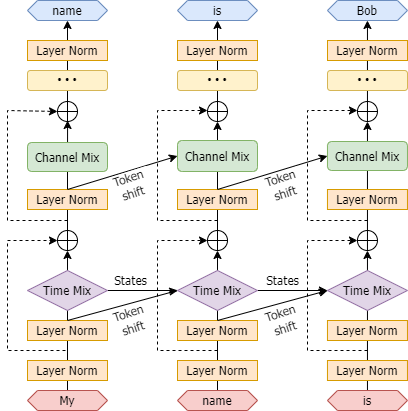
\includegraphics[scale=0.5]{Figures/RWKV-arch.png}
      \caption{معماری \lr{RWKV} برای مدل های زبانی}
      \vspace{0.7em}
      \caption*{گرفته شده از \cite{RWKV}}
      \label{Fig:RWKV}
\end{figure}

\begin{figure}%
      \centering
      \subfloat[\centering \lr{Residual block} \label{fig:RWKVB}]{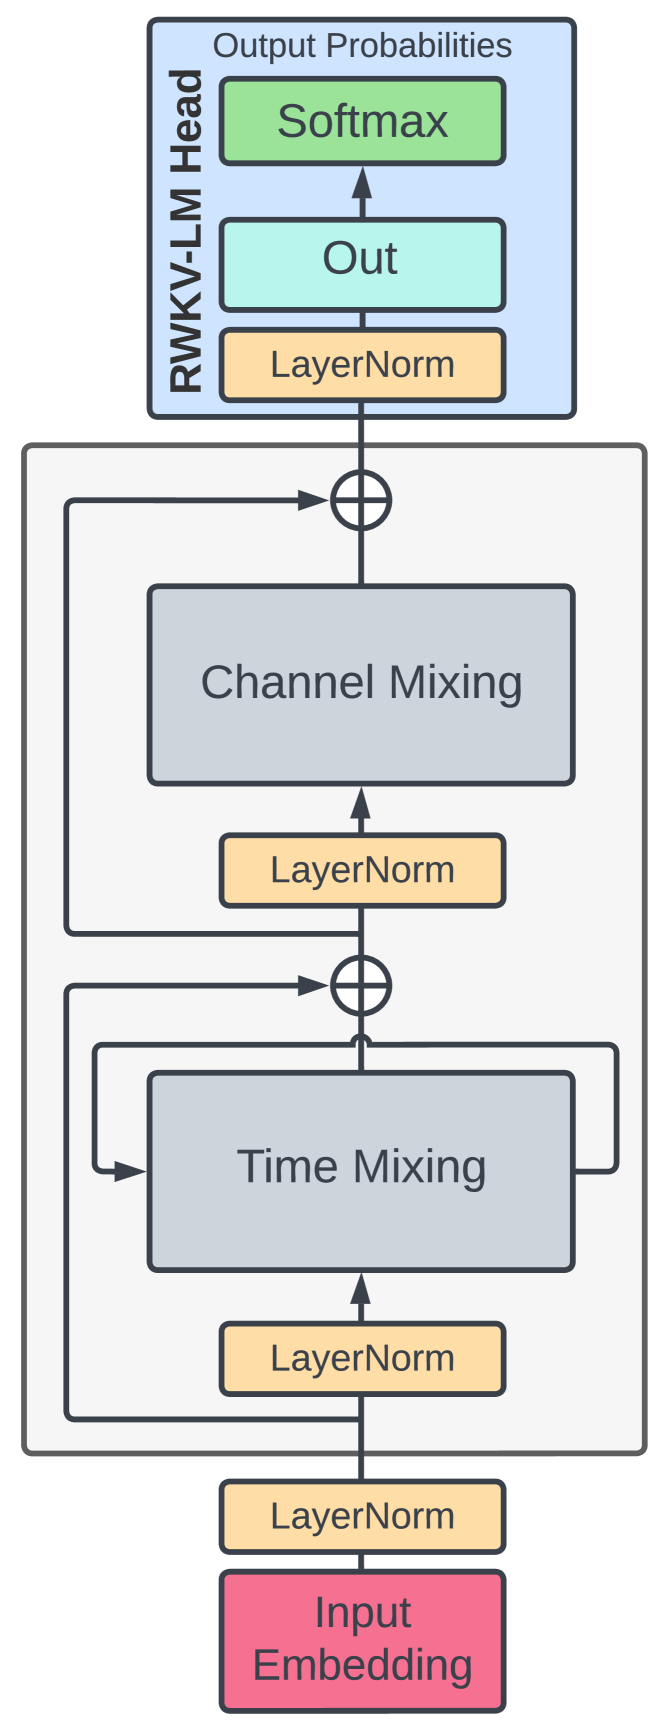
\includegraphics[scale=0.15]{Figures/x3.png} }%
      \qquad
      \subfloat[\centering \lr{Final head of language model} \label{fig:RWKVC}]{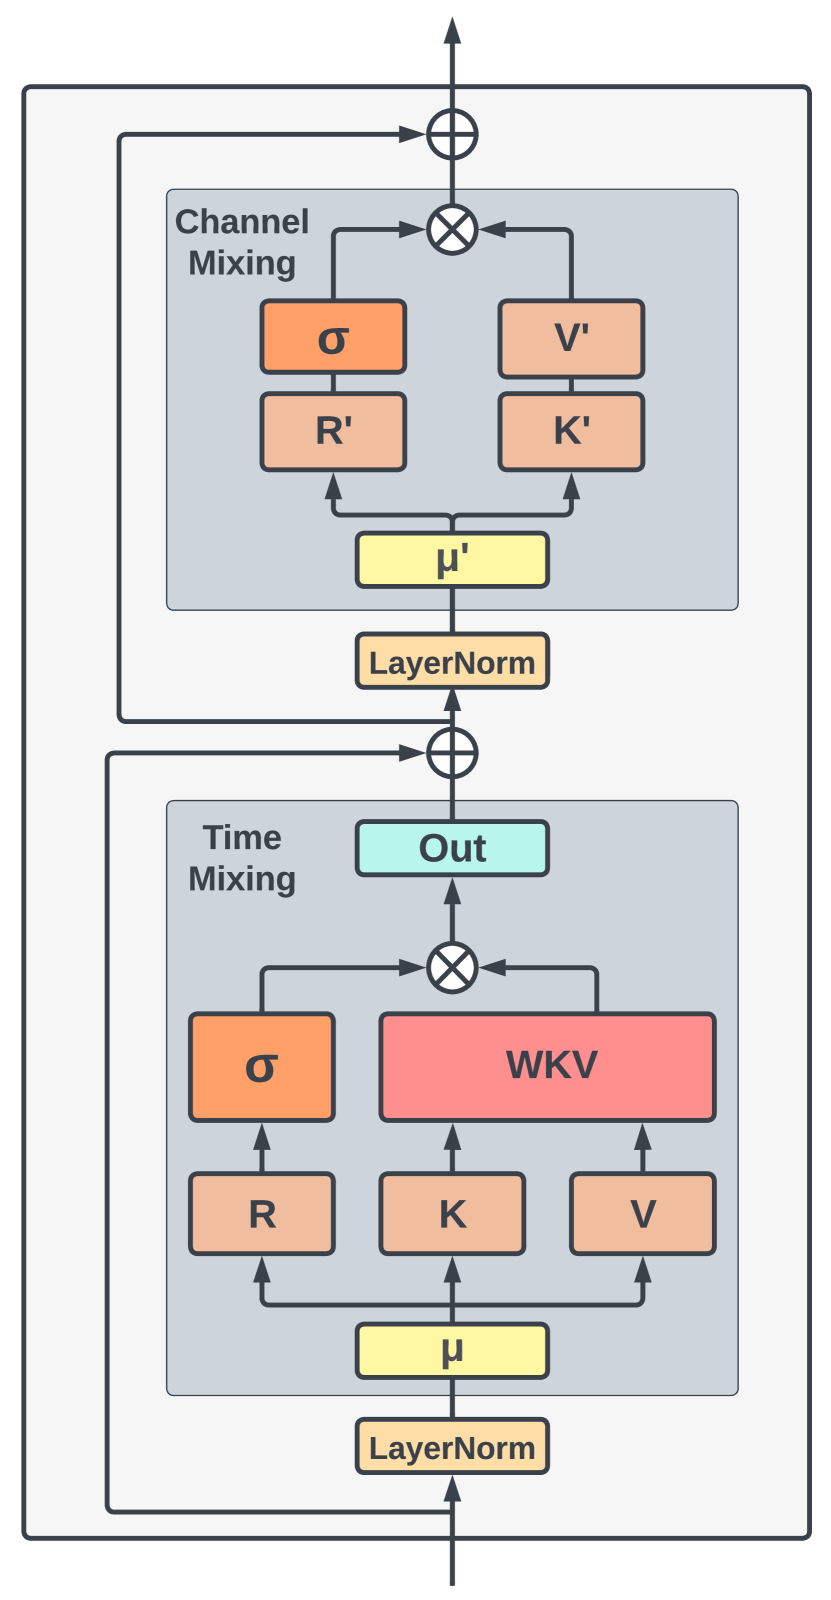
\includegraphics[scale=0.15]{Figures/x2.png} }%
      \caption{عناصر موجود در یک بلوک \lr{RWKV}}
      \vspace{0.7em}
      \caption*{گرفته شده از \cite{RWKV}}
      \label{fig:RWKVBocks}
      %
\end{figure}


\subsubsection{\lr{RWKV} در مقایسه با \lr{Transformer}}
در مورد آموزش یک مدل زبانی برای تولید موسیقی لو-فای، ما تصمیم گرفتیم از معماری \lr{RWKV} به جای معماری ترانسفورمر استفاده کنیم. یکی از دلایل اصلی این انتخاب این است که \lr{RWKV} برای کارایی بیشتر و اجرای آسان‌تر روی \lr{CPU} طراحی شده است که برای پروژه ما مفید است.

با توجه به \xt{tab:inference_complexity} می‌تواند گفت \lr{RWKV} می‌تواند در استنتاج بهتر از ترانسفورمرها باشد زیرا پیچیدگی محاسباتی کمتری در زمان و فضا دارد. به طور خاص، \lr{RWKV} دارای پیچیدگی زمانی $O(Td)$ و پیچیدگی فضایی $O(d)$ است، در حالی که ترانسفورمرها دارای پیچیدگی زمانی $O(T^2d)$ و پیچیدگی فضایی $O(T^2 + Td)$ هستند.
این بدان معناست که با افزایش طول دنباله ورودی $T$ ، هزینه محاسباتی \lr{RWKV} به صورت خطی با $T$ افزایش می‌یابد، در حالی که هزینه محاسباتی ترانسفورمرها به صورت درجه دوم با $T$ افزایش می‌یابد. این امر \lr{RWKV} را برای استنتاج و آموزش دنباله‌های طولانی کارآمدتر می‌کند.

علاوه بر این، پیچیدگی فضایی \lr{RWKV} $O(d)$ است که کمتر از پیچیدگی فضایی ترانسفورمرها $O(T^2 + Td)$ است. این بدان معناست که \lr{RWKV} به حافظه کمتری برای ذخیره وزن‌ها و فعال‌سازی‌های مدل نیاز دارد که می‌تواند برای آموزش و استنتاج در دستگاه‌هایی با حافظه محدود مفید باشد.

به طور کلی، نیازهای محاسباتی و حافظه کمتر \lr{RWKV} آن را به انتخاب کارآمدتری نسبت به ترانسفورمرها برای استنتاج، به ویژه برای دنباله‌های طولانی تبدیل می‌کند.

\begin{table}
      \centering
      \caption{مقایسه پیچیدگی استنتاج \lr{RWKV} با ترانسفورمرهای مختلف}
      \caption*{در اینجا $T$ طول دنباله، $d$ ‌بُعد ویژگی‌ها است.}
      \label{tab:inference_complexity}
      \begin{tabular}{|l|c|c|}
            \hline
            \multicolumn{1}{|c|}{\textbf{مدل}}                            & \multicolumn{1}{c|}{\textbf{پیچیدگی زمانی}} & \multicolumn{1}{c|}{\textbf{پیچیدگی فضایی}} \\
            \hline
            \lr{Transformer}                                              & $O(T^2d)$                                   & $O(T^2 + Td)$                               \\
            \lr{Linear Transformers \cite{katharopoulos2020transformers}} & $O(Td^2)$                                   & $O(Td + d^2)$                               \\
            \lr{RWKV}                                                     & $O(Td)$                                     & $O(d)$                                      \\
            \hline
      \end{tabular}
\end{table}

علاوه بر این، \lr{RWKV} یک مکانیزم توجه \LTRfootnote{Attention mechanism} را در خود جای داده است که به مدل اجازه می‌دهد هنگام تولید توکن بعدی، بر روی بخش‌های خاصی از دنباله ورودی تمرکز کند. این مکانیزم به \lr{RWKV} امکان می‌دهد تا وابستگی‌ها و روابط بلندمدت بین توکن‌ها را به دست آورد، در حالی که همچنان کارایی یک مدل ترتیبی را حفظ می‌کند. مکانیزم توجه در \lr{RWKV} به گونه‌ای طراحی شده است که از نظر محاسباتی کارآمد باشد و از ترکیبی از تبدیل‌های خطی و ضرب نقطه‌ای برای محاسبه وزن‌های توجه استفاده کند.

معماری \lr{RWKV} .به طور خاص برای پردازش داده‌های جریانی طراحی شده است. \lr{RWKV} داده‌های ورودی را به صورت جریانی پردازش می‌کند، به طوری که هر توکن ورودی به محض ورود پردازش می‌شود، بدون نیاز به بارگذاری کل دنباله ورودی در حافظه. این به \lr{RWKV} اجازه می‌دهد تا دنباله‌های ورودی بزرگ، مانند آهنگ‌ها یا فایل‌های صوتی طولانی، را بدون تمام شدن حافظه مدیریت کند.

به طور کلی، معماری \lr{RWKV} تعادلی بهتر بین عملکرد، کارایی و سهولت استقرار فراهم می‌کند و آن را به یک انتخاب ایده‌آل برای تولید موسیقی لو-فای تبدیل می‌کند.


\subsection{فرمت فایل \lr{MIDI}}

فرمت \lr{MIDI} \LTRfootnote{Musical Instrument Digital Interface} \cite{de2017understanding} یک استاندارد فنی برای ارتباط بین ابزارهای موسیقی الکترونیکی، کامپیوترها و دیگر دستگاه‌های مرتبط با موسیقی است. برخلاف فایل‌های صوتی معمولی مانند \lr{MP3} یا \lr{WAV}، فایل‌های \lr{MIDI} حاوی داده‌های صوتی واقعی نیستند. آن‌ها شامل اطلاعاتی مانند نت‌های موسیقی، زمان‌بندی، مدت زمان و شدت صدا برای هر نت هستند.

این فرمت به موسیقی‌دانان و تولیدکنندگان موسیقی اجازه می‌دهد تا داده‌های موسیقی را به صورت دیجیتالی ضبط و پخش کنند و به راحتی بین نرم‌افزارها و سخت‌افزارهای مختلف به اشتراک بگذارند. به دلیل اندازه کوچک فایل‌های \lr{MIDI}، انتقال و ذخیره‌سازی آن‌ها بسیار آسان است.

از دیدگاه کامپیوتری، فایل‌های \lr{MIDI} به عنوان مجموعه‌ای از پیام‌های دیجیتالی ذخیره می‌شوند که هر پیام شامل اطلاعاتی درباره نحوه پخش موسیقی است. این پیام‌ها به صورت باینری کدگذاری می‌شوند و شامل سه بخش اصلی هستند:

\begin{enumerate}
      \def\labelenumi{\arabic{enumi}.}
      \item
            \textbf{پیام‌های وضعیت \LTRfootnote{Status Messages}}: این پیام‌ها نوع عملیاتی که
            باید انجام شود را مشخص می‌کنند، مانند نواختن یک نت، تغییر شدت صدا، یا
            تغییر ابزار موسیقی.
      \item
            \textbf{پیام‌های داده \LTRfootnote{Data Messages}}: این پیام‌ها اطلاعات دقیق‌تری
            درباره عملیات مشخص شده در پیام‌های وضعیت ارائه می‌دهند، مانند شماره نت،
            شدت صدا، و مدت زمان.
      \item
            \textbf{زمان‌بندی \LTRfootnote{Timing}}: این بخش زمان دقیق اجرای هر پیام را مشخص
            می‌کند، که به دستگاه‌ها اجازه می‌دهد تا موسیقی را با دقت زمانی بالا پخش
            کنند.
\end{enumerate}

\begin{example}[]
      \centering
      \label{example:}
      پیام وضعیت برای نواختن نت: \texttt{Note On}

      داده پیام می‌تواند شماره نت باشد مثل  \lr{C4} یا شدت صدا 64

      زمان‌بندی: زمان شروع مثلاً 500 میلی‌ثانیه پس از شروع

      این پیام‌ها به ترتیب در یک فایل \lr{MIDI} ذخیره می‌شوند و هنگام پخش، دستگاه‌های \lr{MIDI} این پیام‌ها را تفسیر کرده و
      موسیقی را تولید می‌کنند. این ساختار به کامپیوترها و دستگاه‌های موسیقی اجازه می‌دهد تا به صورت هماهنگ و دقیق موسیقی را پخش کنند.

\end{example}


\begin{figure}[!htb]
      \centering
      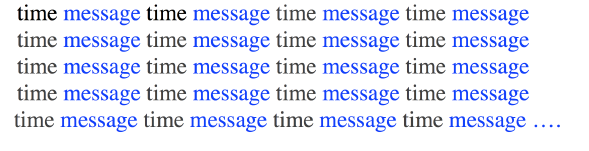
\includegraphics[scale=1]{Figures/Screenshot 2024-08-29 021655.png}
      \caption{ساختار فایل \lr{MIDI}
      }
      \label{Fig:MIDI}
\end{figure}

استفاده از فرمت \lr{MIDI} برای آموزش مدل‌های زبانی نسبت به فرمت \lr{WAV} بهتر است زیرا:

\begin{enumerate}
      \def\labelenumi{\arabic{enumi}.}
      \item
            \textbf{اندازه فایل کوچکتر}: فایل‌های \lr{MIDI} بسیار کوچکتر از فایل‌های \lr{WAV}
            هستند. این امر باعث می‌شود که پردازش و انتقال داده‌ها سریع‌تر و کارآمدتر
            باشد.
      \item
            \textbf{داده‌های ساختاریافته}: فایل‌های \lr{MIDI} شامل اطلاعات دقیق و
            ساختاریافته‌ای درباره نت‌های موسیقی، زمان‌بندی، و شدت صدا هستند. این
            داده‌ها به مدل‌های زبانی کمک می‌کنند تا الگوهای موسیقی را بهتر درک کنند و
            پیش‌بینی‌های دقیق‌تری انجام دهند.
      \item
            \textbf{انعطاف‌پذیری بیشتر}: با استفاده از \lr{MIDI}، می‌توان به راحتی
            تغییرات مختلفی در موسیقی اعمال کرد، مانند تغییر تمپو، کلید، و ابزار
            موسیقی. این انعطاف‌پذیری به مدل‌های زبانی کمک می‌کند تا با شرایط مختلف
            سازگار شوند و عملکرد بهتری داشته باشند.
      \item
            \textbf{کاهش نویز}: فایل‌های \lr{WAV} شامل داده‌های صوتی خام هستند که ممکن
            است نویز و اختلالات زیادی داشته باشند. در مقابل، فایل‌های \lr{MIDI} تنها
            شامل داده‌های دیجیتالی هستند که نویز ندارند و این امر باعث می‌شود که
            مدل‌های زبانی با داده‌های تمیزتر و دقیق‌تری آموزش ببینند.
\end{enumerate}

یک مزیت دیگر استفاده از فرمت \lr{MIDI} برای آموزش مدل‌های زبانی این است که موسیقی چندلایه را به خوبی پشتیبانی می‌کند. فایل‌های \lr{MIDI} می‌توانند چندین ترک \LTRfootnote{Track} را به صورت همزمان ذخیره کنند، که هر ترک می‌تواند نمایانگر یک ابزار موسیقی مختلف باشد. این ویژگی به مدل‌های زبانی اجازه می‌دهد تا تعاملات پیچیده بین سازهای مختلف را درک کنند و تحلیل کنند که چگونه این سازها با هم ترکیب می‌شوند تا یک قطعه موسیقی کامل را تشکیل دهند.

\section{روشهای پيشين}
\subsection{استفاده از معماری \lr{VAE}}
پروژه \lr{jacbz/Lofi} \cite{Zhang} با استفاده از معماری \lr{VAE} کار مشابهی را انجام می دهد.
استفاده از معماری \lr{RWKV}، معماری که ما در این پروژه استفاده کرده‌ایم، برای ساخت موزیک
ﻟﻮ-ﻓﺎﻱ \LTRfootnote{Lo-Fi} مزایای متعددی نسبت به \lr{VAE} \LTRfootnote{Variational Autoencoder} دارد:

\begin{itemize}
      \def\labelenumi{\arabic{enumi}.}
      \item
            \textbf{حفظ ساختار زمانی}: \lr{RWKV} به دلیل استفاده از مکانیزم‌های بازگشتی،
            قادر است ساختار زمانی و توالی‌های طولانی را بهتر حفظ کند. این ویژگی
            برای موزیک ﻟﻮ-ﻓﺎﻱ که اغلب دارای الگوهای تکراری و ریتمیک است، بسیار مهم
            است.
      \item
            \textbf{کیفیت بازسازی بهتر}: \lr{RWKV} به دلیل استفاده از مکانیزم توجه، می‌تواند جزئیات بیشتری از داده‌های ورودی را حفظ کند و بازسازی
            دقیق‌تری ارائه دهد.
      \item
            \textbf{انعطاف‌پذیری بیشتر}: این معماری به دلیل استفاده از مکانیزم‌های
            توجه \LTRfootnote{Attention mechanism}، می‌تواند به طور دینامیک به بخش‌های مختلف داده توجه کند و این امر
            باعث می‌شود که در تولید موزیک‌های پیچیده‌تر و متنوع‌تر عملکرد بهتری داشته
            باشد.
\end{itemize}

پروژه \lr{jacbz/Lofi} شامل چندین محدودیت است. یکی از محدودیت‌های اصلی این پروژه این است که به دلیل استفاده از فضای نهان \LTRfootnote{Latent space} با ابعاد کمتر، ممکن است در بازسازی آهنگ‌های طولانی‌تر دچار مشکل شود. این امر می‌تواند منجر به از دست رفتن جزئیات مهم و کاهش کیفیت بازسازی شود. همچنین، \lr{VAE} به دلیل استفاده از توزیع‌های احتمالاتی برای بازسازی داده‌ها، ممکن است در بازسازی جزئیات دقیق دچار مشکل شود و کیفیت نهایی موزیک کاهش یابد.

به طور کلی، معماری \lr{RWKV} به دلیل توانایی بهتر در حفظ ساختار زمانی و جزئیات داده‌ها، برای ساخت موزیک ﻟﻮ-ﻓﺎﻱ مناسب‌تر است. از طرف دیگر، \lr{VAE} به دلیل محدودیت‌های ذاتی خود در بازسازی آهنگ‌های طولانی و پیچیده، ممکن است کیفیت نهایی موزیک را کاهش دهد.

\subsection{استفاده از شبکه‌های حافظه طولانی کوتاه مدت}
پروژه \lr{MR-KARPIN/lofi-LSTM} \cite{mrkarpin_2023_github} با استفاده از شبکه‌های حافظه طولانی کوتاه مدت \LTRfootnote{Long Short-Term Memory} کار مشابهی را انجام می‌دهد. که استفاده از معماری
استفاده از معماری \lr{RWKV} برای ساخت موزیک ﻟﻮ-ﻓﺎﻱ مزایای متعددی نسبت به شبکه‌های حافظه طولانی کوتاه مدت
دارد. \lr{RWKV} به دلیل استفاده از مکانیزم‌ها توجه \LTRfootnote{Attention mechanism}، قادر است ساختار زمانی و توالی‌های طولانی را بهتر حفظ کند. این ویژگی برای موزیک ﻟﻮ-ﻓﺎﻱ که اغلب دارای الگوهای تکراری و ریتمیک است، بسیار مهم است.

از سوی دیگر، یکی از محدودیت‌های اصلی \lr{LSTM} این است که به دلیل استفاده از حافظه کوتاه مدت، ممکن است در بازسازی آهنگ‌های طولانی‌تر دچار مشکل شود. این امر می‌تواند منجر به از دست رفتن جزئیات مهم و کاهش کیفیت بازسازی شود.

به طور کلی، معماری \lr{RWKV} به دلیل توانایی بهتر در حفظ ساختار زمانی و جزئیات داده‌ها، برای ساخت موزیک ﻟﻮ-ﻓﺎﻱ مناسب‌تر است. از طرف دیگر، \lr{LSTM} به دلیل محدودیت‌های ذاتی خود در بازسازی آهنگ‌های طولانی و پیچیده، ممکن است کیفیت نهایی موزیک را کاهش دهد.

\subsection{جمع بندی}
معماری \lr{RWKV} یک مدل شبکه عصبی است که مزایای شبکه‌های عصبی بازگشتی و ترانسفورمرها را برای پردازش کارآمد داده‌های دنباله‌ای ترکیب می‌کند. برخلاف شبکه‌های عصبی بازگشتی که به دلیل مشکلاتی مانند ناپدید شدن گرادیان با وابستگی‌های بلندمدت مشکل دارند، \lr{RWKV} این وابستگی‌ها را حفظ کرده و از قابلیت‌های پردازش موازی ترانسفورمرها بهره می‌برد. این رویکرد ترکیبی به \lr{RWKV} اجازه می‌دهد تا به صورت موازی مانند ترانسفورمرها آموزش ببیند اما در زمان استنتاج به صورت دنباله‌ای عمل کند، که این ویژگی آن را بهترین گزینه برای پروژه ما می‌کند.